\documentclass{article}
\usepackage{graphicx} % Required for inserting images
\usepackage{geometry}
\usepackage{amsmath}
\usepackage{svg}
\usepackage{todonotes}
\usepackage{hyperref}
\usepackage{bm}

\title{Drone Stabilization}
\author{Matthew \& friends}
\date{April 2025}

\begin{document}

\maketitle

\section*{Setting up the model}
We denote the state of a quadcopter drone in terms of its position and state as 

$$
\mathbf{s}(t) = \big(x(t), y(t), z(t), \phi(t), \theta(t), \psi(t) \big)
$$

where $(x, y, z)$ represents the position of the center of the drone, and $(\phi, \theta, \psi)$ represents the orientation of the drone in terms of its Tait-Bryan angles, a set of three angles that describes the orientation where $(\phi, \theta, \psi) = \mathbf{0}$ means the drone is not tilted and points north.

\begin{figure}[h]
    \centering
    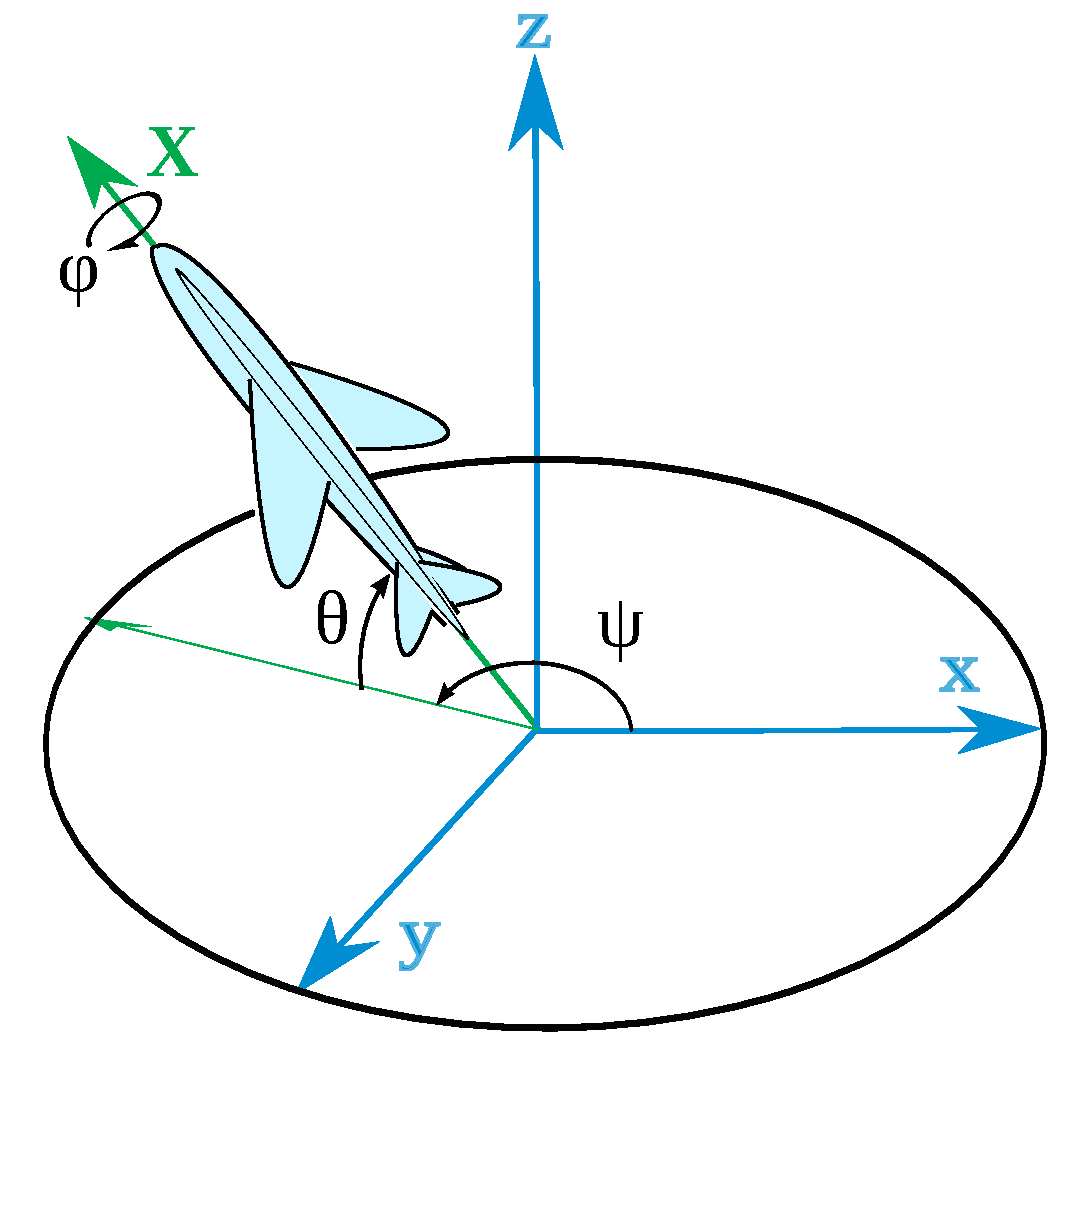
\includegraphics[width=0.4\textwidth]{Plane_with_ENU_embedded_axes.pdf}
    \caption{Tait-Bryan angles we're using (just imagine a drone instead of a plane!)}
\end{figure}

We denote our control over the speed rotors of the drone with 

$$
\mathbf{u} = \big(u_1(t), u_2(t), u_3(t), u_4(t)\big)
$$

\todo{Explain u}


We set a fixed final time $t_f$ and seek to control the drone via the cost functional

$$
J(\mathbf{u}) = \int_{0}^{t_f}\Big( \Vert \mathbf{u} \Vert_2^2 + \alpha \Vert \mathbf{s} \Vert_2^2 \Big) dt
$$

where $\alpha > 0$ weights our hopes to quickly stabilize the drone versus save energy.

We set $\mathbf{s}(0)$ to be some arbitrary $\mathbf{s}_0$ and allow $\mathbf{s}(t_f)$ to be free, allowing the cost functional to ensure that our state remains stable.

\section*{State evolution}

We proceed to describe how the control interacts with the state of the drone.

\todo{Add Newton-Euler equations}

We make the assumption that the angular velocity is always small, allowing us to ignore the last term.

The force on the drone from its rotors when $(\phi, \theta, \psi) = \mathbf{0}$ is simply 

$$
\begin{pmatrix}
    0 \\ 0 \\ \sum_{i=1}^4 u_i
\end{pmatrix}
$$

since the rotors thrust upward relative to the drone. 

In the same orientation, the torque on the drone is 

$$
\begin{pmatrix}u_2 - u_4 \\ u_3 - u_1 \\ \lambda(u_1 + u_3 - u_2 - u_4) \end{pmatrix}
$$

with $\lambda >0$, since two of the rotors spin clockwise and the other two spin counter-clockwise, causing a bit of torque rotating the drone. \todo{Explain further}

Now we need to be able to express this force no matter what the orientation of the drone is. We use the following rotation matrices described in \href{https://en.wikipedia.org/wiki/Davenport_chained_rotations}{this Wikipedia article on the subject}:

\[
R_x(\phi) = \text{Roll}(\phi) =
\begin{bmatrix}
1 & 0 & 0 \\
0 & \cos\phi & -\sin\phi \\
0 & \sin\phi & \cos\phi
\end{bmatrix}
\]

\[
R_y(\theta) = \text{Pitch}(\theta) =
\begin{bmatrix}
\cos\theta & 0 & \sin\theta \\
0 & 1 & 0 \\
-\sin\theta & 0 & \cos\theta
\end{bmatrix}
\]

\[
R_z(\psi) = \text{Yaw}(\psi) =
\begin{bmatrix}
\cos\psi & -\sin\psi & 0 \\
\sin\psi & \cos\psi & 0 \\
0 & 0 & 1
\end{bmatrix}
\]

The matrix of the composed rotations is

\[
R = \text{Yaw}(\psi)\, \text{Pitch}(\theta)\, \text{Roll}(\phi) 
= R_z(\psi) R_y(\theta) R_x(\phi).
\]

We can express the force and torque on the drone at an arbitrary orientation with $R$ and $g$ as a gravitational constant:

\[
\begin{aligned}
    \mathbf{F} &= R(\phi, \theta, \psi) \begin{pmatrix} 
        0 \\ 
        0 \\ 
        \sum_{i} u_i - g
    \end{pmatrix} \\
    \bm{\tau} &= R(\phi, \theta, \psi) \begin{pmatrix}
        u_2 - u_4 \\ 
        u_3 - u_1 \\ 
        \lambda(u_1 + u_3 - u_2 - u_4) 
    \end{pmatrix}
\end{aligned}
\]

Now we are ready to model the evolution of the state of the drone. The Newton-Euler equations extend the classic relationship $F = m a$ into three dimensions and add in torque and gyroscopic effects for a moving object.

\begin{equation*}
\begin{pmatrix}
    \bm{F} \\
    \bm{\tau}
    \end{pmatrix}
    =
    \begin{pmatrix}
    m I & 0 \\
    0 & \mathcal{I}
    \end{pmatrix}
    \ddot{\bm{s}}
    +
    \begin{pmatrix}
    0 \\
    \bm{\omega} \times \mathcal{I} \bm{\omega}
\end{pmatrix}
\end{equation*}

where $m$ is the mass of the object, $I$ is a $3 \times 3$ identity matrix, $\mathcal{I}$ is a diagonal matrix representing the moment of inertia of the object, and $\bm{\omega} = (\dot{\phi}, \dot{\theta}, \dot{\psi})$.

We assume the angular velocity $\bm{\omega}$ (we hope the drone is not rapidly flipping end over end or spinning like a top), reorganize the equation, and plug in our model for $\bm{F}$ and $\bm{\tau}$ to yield the state evolution equation

\begin{equation}
\ddot{\mathbf{s}} = 
\begin{pmatrix}
    m I & \mathbf{0} \\
    \mathbf{0} & \mathcal{I}
\end{pmatrix}^{-1}
\begin{pmatrix}
    \bm{F} \\
    \bm{\tau}
\end{pmatrix}
= \begin{pmatrix}
    m I & \mathbf{0} \\
    \mathbf{0} & \mathcal{I}
\end{pmatrix}^{-1}
\begin{pmatrix}
    R(\phi, \theta, \psi) \begin{pmatrix} 
        0 \\ 
        0 \\ 
        \sum_{i} u_i
    \end{pmatrix} \\
    R(\phi, \theta, \psi) \begin{pmatrix}
        u_2 - u_4 \\ 
        u_3 - u_1 \\ 
        \lambda(u_1 + u_3 - u_2 - u_4) 
    \end{pmatrix}
\end{pmatrix}
\label{eq:SecondOrderState}
\end{equation}

\section*{Reducing to first-order system}

The state evolution equation described above is second-order. We hope to work with a first order system, so we define

$$
\bm{\sigma} 
= \begin{pmatrix} \bm{\sigma}_1 \\ \bm{\sigma}_2 \end{pmatrix}
= \begin{pmatrix} \bm{s} \\ \dot{\bm{s}} \end{pmatrix}
= (x, y, z, \phi, \theta, \psi, \dot{x}, \dot{y}, \dot{z}, \dot{\phi}, \dot{\theta}, \dot{\psi})
$$

and observe that 

\[
\dot{\sigma} 
= \begin{pmatrix} \dot{\bm{\sigma}}_1 \\ \dot{\bm{\sigma}}_2 \end{pmatrix}
= \begin{pmatrix} \dot{\bm{s}} \\ \ddot{\bm{s}} \end{pmatrix} 
= \begin{pmatrix} \bm{\sigma}_2 \\ \ddot{\bm{s}} \end{pmatrix}
\]

with $\ddot{\bm{s}}$ as in Equation \ref{eq:SecondOrderState}. This first order equation is the equation we will work with in what follows, thus thinking of the ``state'' as the 12-dimensional $\bm{\sigma}$ encoding both translational and angular position and velocity.

\section*{Deriving optimal control}

We now set up the Hamiltonian $H$ and solve for the optimal control. Let $\bm{p}(t)$ be the 12-dimensional costate evolving alongside $\bm{\sigma}(t)$.

\begin{equation*}
    H = \bm{p} \cdot \dot{\bm{\sigma}} - \Big( \Vert \mathbf{u} \Vert_2^2 + \alpha \Vert \mathbf{s} \Vert_2^2 \Big)
\end{equation*}

Since $\bm{u}$ maximizes $H$,

\begin{equation}
\begin{aligned}
    0 
    &= \frac{\partial H}{\partial \bm{u}} \\
    &= \bm{p} \cdot \frac{\partial}{\partial \bm{u}} \dot{\bm{\sigma}}
        - \frac{\partial}{\partial \bm{u}} \Vert \bm{u} \Vert_2^2
        - \alpha \frac{\partial}{\partial \bm{u}} \Vert \bm{s} \Vert_2^2 \\
    &= \bm{p} \cdot \frac{\partial}{\partial \bm{u}} \dot{\bm{\sigma}}
        - 2 \bm{u}
        - 0 \\
    &\implies \bm{u} = \frac{1}{2} \Big( \bm{p} \cdot \frac{\partial}{\partial \bm{u}} \dot{\bm{\sigma}} \Big)
\end{aligned}\begin{pmatrix}
    m I & \mathbf{0} \\
    \mathbf{0} & \mathcal{I}
\end{pmatrix}^{-1}
\begin{pmatrix}
    R(\phi, \theta, \psi) \begin{pmatrix} 
        0 \\ 
        0 \\ 
        \sum_{i} u_i
    \end{pmatrix} \\
    R(\phi, \theta, \psi) \begin{pmatrix}
        u_2 - u_4 \\ 
        u_3 - u_1 \\ 
        \lambda(u_1 + u_3 - u_2 - u_4) 
    \end{pmatrix}
\end{pmatrix}
\end{equation}

We need to calculate $ \frac{\partial}{\partial \bm{u}} \dot{\bm{\sigma}} $. Let $i \in \{1, \ldots, 12\}$.
\begin{equation}
\begin{aligned}
    \frac{\partial}{\partial u_i} \dot{\bm{\sigma}} 
    &= \frac{\partial}{\partial u_i} \begin{pmatrix} \bm{\sigma}_2 \\ \ddot{\bm{s}} \end{pmatrix} \\
    &= \begin{pmatrix}
        0 \\
        0 \\
        0 \\
        0 \\
        0 \\
        0 \\
        \frac{\partial}{\partial u_i} \begin{pmatrix}
            m I & \mathbf{0} \\
            \mathbf{0} & \mathcal{I}
        \end{pmatrix}^{-1}
        \begin{pmatrix}
            R(\phi, \theta, \psi) \begin{pmatrix} 
                0 \\ 
                0 \\ 
                \sum_{i} u_i
            \end{pmatrix} \\
            R(\phi, \theta, \psi) \begin{pmatrix}
                u_2 - u_4 \\ 
                u_3 - u_1 \\ 
                \lambda(u_1 + u_3 - u_2 - u_4) 
            \end{pmatrix}
        \end{pmatrix}
    \end{pmatrix} \\
    &= \begin{pmatrix}
        0 \\
        0 \\
        0 \\
        0 \\
        0 \\
        0 \\
        \begin{pmatrix}
            m I & \mathbf{0} \\
            \mathbf{0} & \mathcal{I}
        \end{pmatrix}^{-1}
        \begin{pmatrix}
            R(\phi, \theta, \psi) \begin{pmatrix} 
                0 \\ 
                0 \\ 
                \frac{\partial}{\partial u_i} \sum_{i} u_i
            \end{pmatrix} \\
            R(\phi, \theta, \psi) \frac{\partial}{\partial u_i} \begin{pmatrix}
                u_2 - u_4 \\ 
                u_3 - u_1 \\ 
                \lambda(u_1 + u_3 - u_2 - u_4) 
            \end{pmatrix}
        \end{pmatrix}
    \end{pmatrix} \\
    &= \begin{pmatrix}
        0 \\
        0 \\
        0 \\
        0 \\
        0 \\
        0 \\
        \begin{pmatrix}
            m I & \mathbf{0} \\
            \mathbf{0} & \mathcal{I}
        \end{pmatrix}^{-1}
        \begin{pmatrix}
            R(\phi, \theta, \psi) \begin{pmatrix} 
                0 \\ 
                0 \\ 
                1
            \end{pmatrix} \\
            R(\phi, \theta, \psi) \frac{\partial}{\partial u_i} \begin{pmatrix}
                u_2 - u_4 \\ 
                u_3 - u_1 \\ 
                \gamma_i
            \end{pmatrix}
        \end{pmatrix}
    \end{pmatrix}
\end{aligned}
\end{equation}

where 

\begin{equation}
    \gamma_i = \begin{cases}
        (0, -1, \lambda) & \text{if } i = 1 \\
        
    \end{cases}
\end{equation}


\end{document}
